\section{Signal to Noise and Spatial Binning}
\label{sec:maps}

\begin{figure}
  \centering
  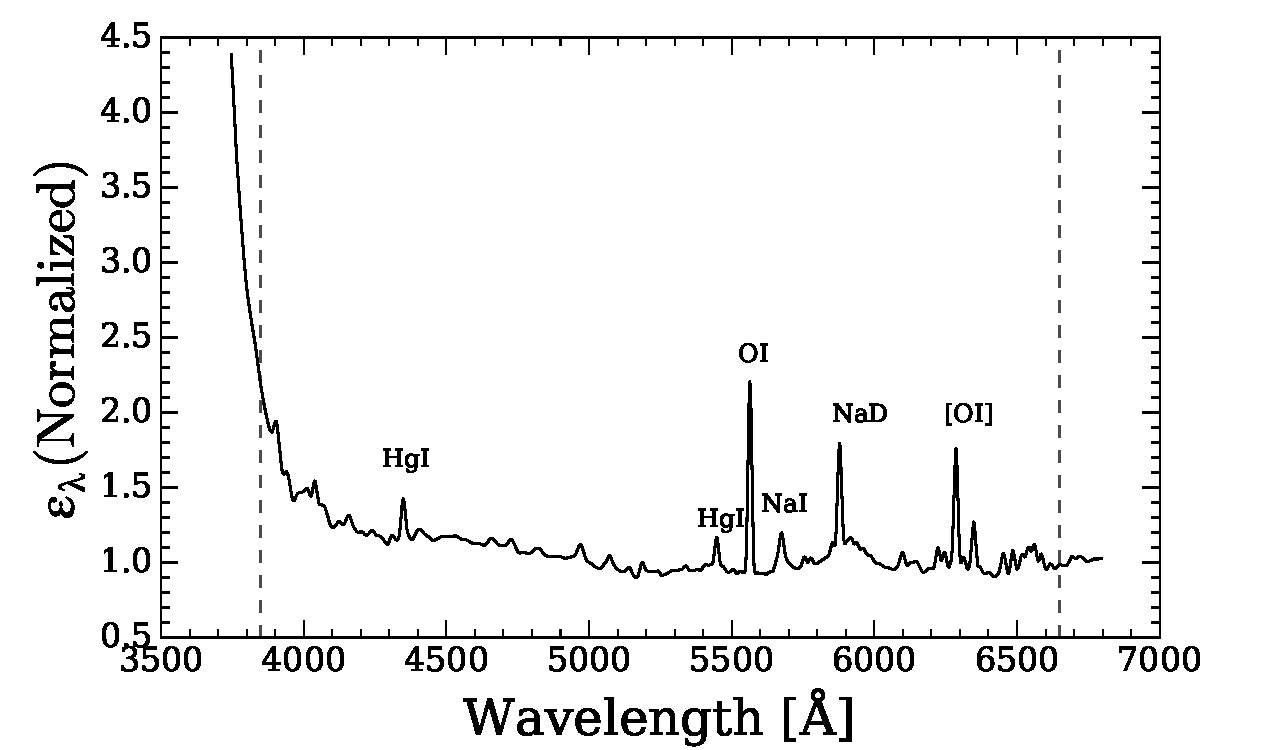
\includegraphics[width=\columnwidth]{891_1/figs/noise_vec.pdf}
  \caption{\label{fig:noise_vec} Characteristic noise vector used to
    construct noisy galaxy models, as described in the text, here
    normalized between \val{5450}{\AA} $\leq \lambda \leq$
    \val{5550}{\AA}. Vertical dashed lines correspond to used spectral
    range in analysis.}
\end{figure}

\subsection{Signal-to-Noise threshold for spectral bins}
\label{sec:snr_threshold}

Despite \GP's design, clumpiness in the distribution of dust and
star-light result in different signal-to-noise ratios (S/N) in each
fiber. Co-adding spectra (``binning'') from adjacent fibers enables us
to homogenize S/N and hence the precision on age and metallicity
inferred from spectral fitting, but at the expense of spatial
resolution. We have attempted to optimize the spectral binning by
defining a critical S/N threshold to achieve a {\it precision} of 10\%
in age and metallicity. In the absence of other mitigating effects,
this precision is ample to detect the vertical age break in a MW-like
heating model and to determine the break height to within 50 pc since
the predicted gradient in light-weigted mean age is very steep near
the mid-plane. At this level of precision, systematic effects in the
interpretation of the break height, e.g., due to inaccuracies of our
estimated line-of-sight depth or model assumptions about star-forming
history become dominant. In what follows we define S/N in pixel units,
where each pixel samples roughly 2\AA.

Accordingly, the critical S/N threshold was determined using an
idealized Monte Carlo simulation of model galaxy spectral energy
distributions (SED) with known star formation histories and
chemistries and therefore known ages and metallicities.  We have
ignored systematic errors in, e.g., flux calibration or between the
model libraries and stellar evolutionary tracks and actuality,
although we address issues with stellar libraries and evolutionary
tracks in Paper II. While other studies have undertaken similar
analyses we stress the importance of this modeling excercise to be
undertaken to any data set distinct in wavelength range and error
vector.

\begin{figure}
  \centering
  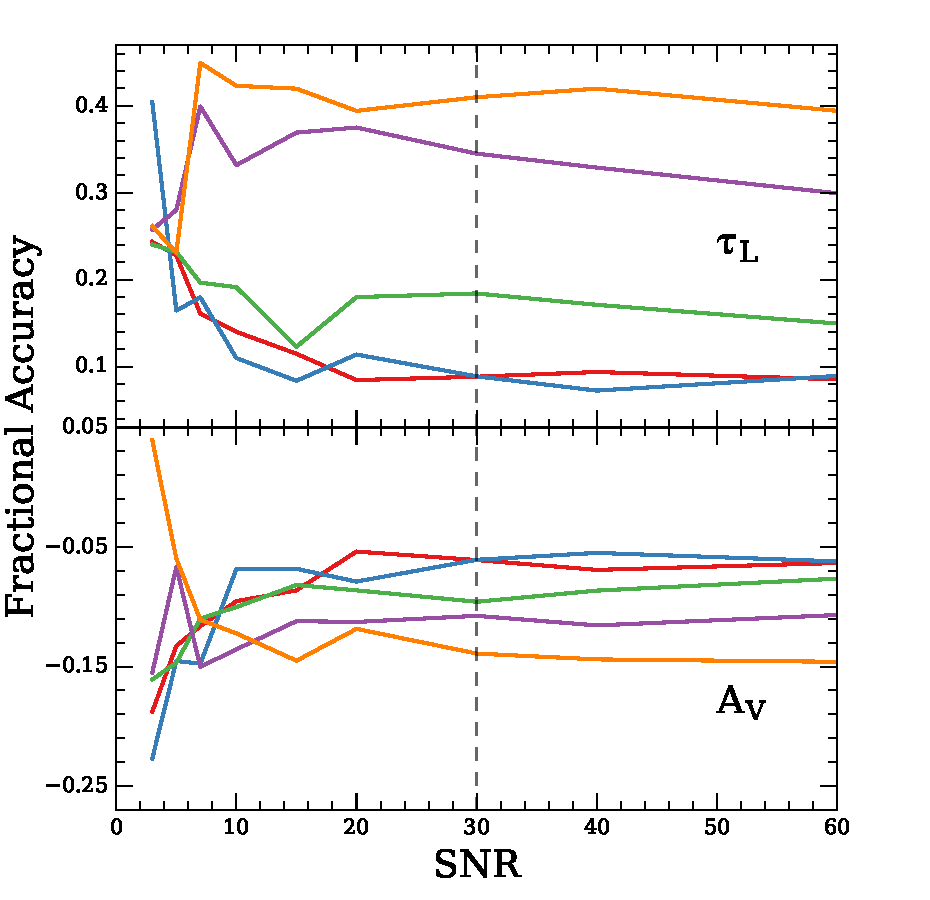
\includegraphics[width=\columnwidth]{891_1/figs/SN_sys.pdf}

  \caption{\label{fig:SN_sys} Systematics in fit parameters caused by
    degeneracies in star formation history as a function of S/N per
    pixel (each pixel samples $\sim 2$\AA).  Fractional accuracy is
    defined as $1 - X_\mathrm{fit}/X_\mathrm{model}$, where $X =
    \tau_L$ in the top panel, and $X = A_V$ in the bottom panel.
    Models adopt a solar-metallicity smoothly declining star-formation
    rate governed by an e-folding time-scale $\tau_{SF}$, while the
    fit has no restrictions on the SFH or metallicity. Colors
    correspond to different values of $\tau_{SF}$ as given in Figure
    \ref{fig:SN_rms}. Vertical dashed lines at S/N=30 pix$^{-1}$) are
    for reference.}
\end{figure}


\begin{figure}
  \centering
  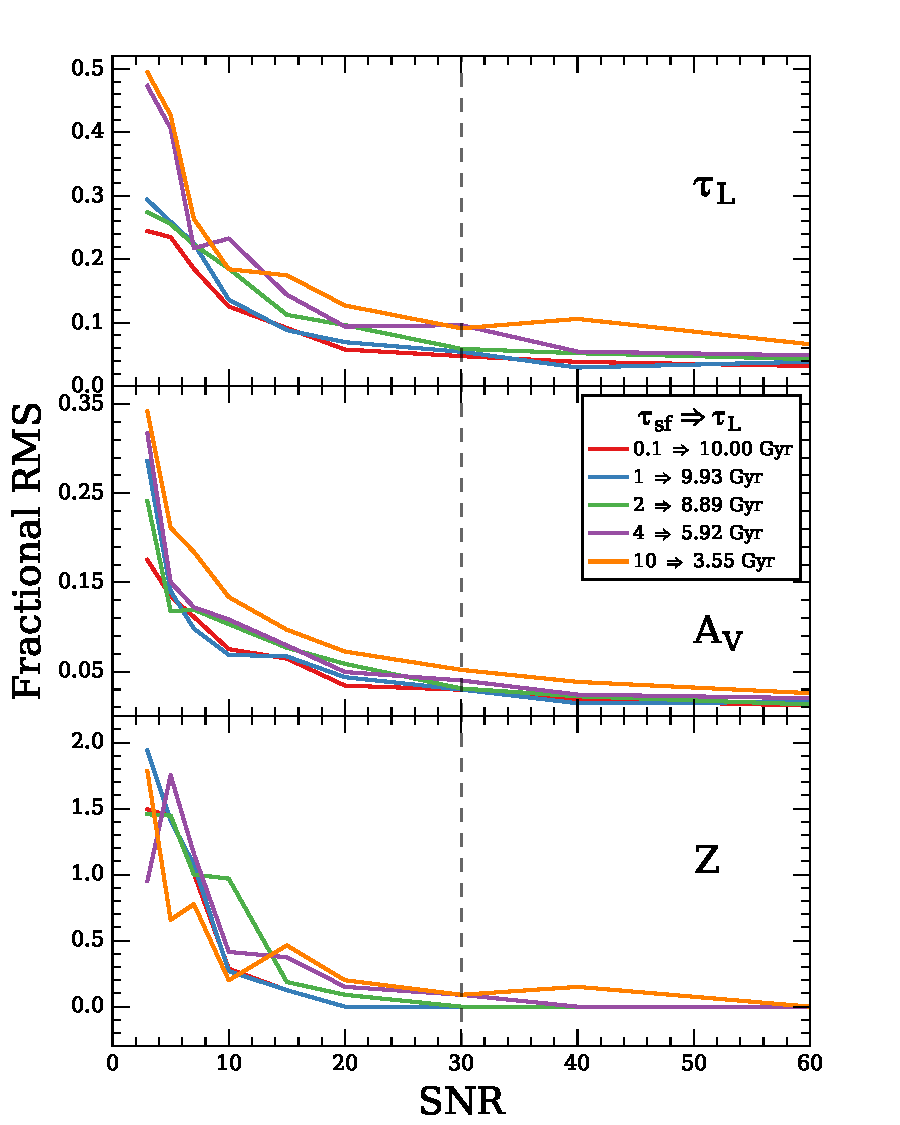
\includegraphics[width=\columnwidth]{891_1/figs/SN_rms.pdf}
  \caption{\label{fig:SN_rms} Precision of recovered parameters as a
    fraction of S/N per pixel for different model input values of mean
    light-weighted age ($\tau_L$, top), extinction ($A_V$, middle),
    and metallicity ($Z$, bottom).  Precision is estimated as the
    root-mean-square deviation of the fitted values from the mean of
    the 30 Monte Carlo noise realizations. Colored lines correspond to
    results for model spectra described in Figure \ref{fig:SN_sys}, as
    indicate in the key. Model values of $\tau_L$ for each $\tau_{SF}$
    assuming a formation epoch 12 Gyr in the past are also
    specified. Vertical dashed lines at S/N = 30 pix$^{-1}$ indicate
    our precision criterion largely driven by $\tau_L$.}
\end{figure}

\subsection{Monte Carlo Simulations}
\label{sec:sims}

Model galaxy spectra were constructed using the method outlined in
Appendix \ref{sec:tau_model} with star-formation e-folding
time-scales, $\tau_{SF}$ = 0.1, 1, 2, 4, and 10 Gyr for a total age of
12 Gyr.  All model galaxies were constructed from mono-metallicity
SSPs with a metallicity of \val{0.4}{\Zsol} and had extinction
dictated by the model of \citet{Charlot00} with $A_V=1.63$ (an optical
depth $\tau_V$ of 1.5, close to the median we in in Paper II from full
spectral fitting). The spectral resolution of the models was set to
210 km s${^-1}$ to match the characteristic resolution of the data at
5500 \AA. For each model galaxy noise was added to produce spectra
with S/N = 3, 5, 7, 10, 15, 20, 30, 40, and 60. We define S/N for both
our galaxy observations and Monte Carlo models as S/N =
$\Sigma_{\lambda}\left(f_\lambda/\epsilon_\lambda\right)/N$ where
$f_\lambda$ is the measured flux, $\epsilon_\lambda$ is the
corresponding error vector, and the sum is over $N$ pixels in a
specified band pass. For our tests we choose the bandpass to be
\val{5450}{\AA} $\leq \lambda \leq$ \val{5550}{\AA}, but we note that
the choice of bandpass only scales the derived S/N thresholds by a
constant related to the SED of our galaxy/models. Provided the
bandpass used to compute the S/N threshold is the same as that used to
bin the data the specific choice of bandpass is irrelevant.

For observed galaxy data the quantities $f_\lambda$ and
$\epsilon_\lambda$ are the result of the reduction described in
section \ref{sec:data_reduction}. For the model galaxies the shape of
$\epsilon_\lambda$ was based on the spectral noise structure of our
data.  To compute $\epsilon_\lambda$ we average together the error
vectors from \emph{all} fibers across all pointings. We then fit a
smooth function to this average to remove high-frequency noise. The
result in Figure \ref{fig:noise_vec} captures the general trend of how
$\epsilon_\lambda$ varies with wavelength in our data.

% {\bf [TODO: A little more discussion and description in the next paragraph 
% is needed. 

% A few things to discuss include:

% Can we say why we think it is reasonable to fit mono-z templates to
% the mono-z simulations? I am thinking about the fact that ultimately
% we expect there to be multi-z stellar pops in N891 and that
% regardless, in the end we fit multi-z models to the data. Do we want
% to know what happens when we allow this degree of freedom in the
% simulations? Will we want to know it when we get back to Paper II?

% Discuss why we are not forcing the fit to have exp SFR, or do we want
% to do that as well? Are we showing anything about this in Paper II? 

For each combination of $\tau_{SF}$ and S/N we generate 30 Monte Carlo
noise realizations (while still maintaining the same S/N) which
produce 30 version of the same galaxy that differ only by stochastic
variations. Once the model galaxies are constructed they are fit using
the same method described in Paper II. In short, a Levenberg-Marquardt
minimization routine is used to fit a superposition of SSPs taken from
the models of \citet{Bruzual03} in the same 10 age bins used by
\citet{Tremonti04} (in Gyr: 0.005, 0.025, 0.1, 0.286, 0.64, 0.904,
1.434.2.5, 5, and 10). The result of each fit is a set of SSP weights
and a single value for extinction $A_V$, assuming the extinction model
of \citet{Charlot00} (i.e., the same extinction model used to
construct the model galaxies). In both the models and the fitting, we
have made the simplifying condition that the same value for the
extinction and the extinction law is applicable to all age stellar
populations; to do otherwise is beyond the scope of this analysis.

When assessing the accuracy and precision of each S/N level we
directly compare the known model $A_V$ to the fit $A_V$, and we use
the mean light-weighted age ($\tau_L$, Equation \ref{eq:MLWA} in
Appendix \ref{sec:tau_model}, as measured between \val{5450}{\AA}
$\leq\lambda\leq$ \val{5550}{\AA})\footnote{ This band-pass for
  definning $\tau_L$ is between and narrowly missing terrestrial and
  airglow lines of HgI and OI. However, since the measurement is made
  from and referenced to the models, night-sky contamination is not
  relevant.}  as a proxy for the SSP weights. This substitution allows
us make a quantitative assessment of the {\it precision} of our fits
but comes with some important caveats concerning {\it accuracy} that
we consider in detail in Paper II, and summarize here.

In the broadest terms $\tau_L$ is known to be degenerate with the
detailed star formation history (SFH); in our models we assume a
smooth, exponentially declining star-formation rate parameterized by
$\tau_{SF}$ but a different SFH could yield a very similar spectrum
with a significantly different $\tau_L$.  Because we do not impose a
specific SFH during the fitting process, our fit values of $\tau_L$
are likely to be systematically offset from the input model values.

More specifically, we find that any model with a smoothly varying
prescription of the SFH (specifically the $\tau_{SF}$ model outlined
in Appendix \ref{sec:tau_model}) gives a generally poor description of
our galaxy spectra and also yield estimates of SFH (via $\tau_L$) that
are offset from the best fitting models with unconstrained star
formation histories. We highlight these systematics in Figure
\ref{fig:SN_sys}.

Fits with unconstrained SFH report values of $\tau_L$ that are offset
by as much as 40\% from the true values of $\tau_{SF}$ model
galaxies. The maximum offsets occur at the largest values of
$\tau_{SF}$, i.e., approaching a constant star-formation rate where
all age SSPs are well represented in the integrated spectrum.  This
suggests systematics may be driven by degeneracies caused by
similarities between the 10 SSPs used during fitting.  In Paper II we
explore methods to reduce the number of SSPs used (and therefore the
number of free parameters) using the statistical methods presented by
\citet{Mosby15}.

\begin{deluxetable}{cccrrrc}
\tablewidth{0.8\textwidth}
\tablecaption{Data Apertures}
\tablehead{
\colhead{Pointing} &
\colhead{Aperture} &
\colhead{Constituent} &
\colhead{S/N} &
\colhead{$r$} &
\colhead{$z$} &
\colhead{Notes}\\
\colhead{Number} &
\colhead{Number} &
\colhead{Fibers} &
\colhead{} &
\colhead{(kpc)} &
\colhead{(kpc)} &
\colhead{}
}
\startdata
1 & 1 & 3, 4, 5, 6, 7, 8 & 32.22 &  4.44 & -0.12 & g\\
1 & 2 & 9, 10, 11, 12, 13, 14, 15, 16, 17 & 26.72 &  5.26 & -0.09 & b\\
1 & 3 & 21 & 34.50 &  4.16 &  0.02 & g\\
1 & 4 & 22, 23, 24, 25, 26, 27 & 31.41 &  4.76 &  0.04 & g\\
1 & 5 & 28, 29, 30 & 14.92 &  5.52 &  0.08 & u\\
1 & 6 & 33, 34, 35, 36, 37, 38, 39 & 30.70 &  4.66 &  0.21 & g
  %% 1 & 7 & 40, 41, 42 & 15.89 &  5.51 &  0.24 & g\\
  %% 1 & 8 & 45, 46, 47, 48 & 30.85 &  4.47 &  0.41 & g\\
  %% 1 & 9 & 49, 50, 51 & 47.30 &  5.24 &  0.44 & g\\
  %% 1 & 10 & 52 & 32.77 &  5.68 &  0.46 & g\\
  %% 1 & 11 & 55, 56, 57, 58, 59 & 43.21 &  4.61 &  0.63 & g\\
  %% 1 & 12 & 60 & 40.73 &  5.45 &  0.67 & g\\
  %% 1 & 13 & 61 & 36.45 &  5.67 &  0.68 & g\\
  %% 1 & 14 & 64, 65 & 48.93 &  4.22 &  0.87 & g\\
  %% 1 & 15 & 66 & 43.20 &  4.62 &  0.89 & g\\
  %% 1 & 16 & 67 & 37.63 &  4.89 &  0.90 & g\\
  %% 1 & 17 & 68 & 39.57 &  5.16 &  0.91 & g\\
  %% 1 & 18 & 69 & 35.57 &  5.43 &  0.92 & g\\
  %% 1 & 19 & 70 & 32.84 &  5.69 &  0.94 & g\\
  %% 1 & 20 & 72 & 36.81 &  4.07 &  1.13 & g\\
  %% 1 & 21 & 73 & 48.06 &  4.34 &  1.15 & g\\
  %% 1 & 22 & 74 & 40.16 &  4.61 &  1.16 & g\\
  %% 1 & 23 & 75 & 39.75 &  4.88 &  1.17 & g\\
  %% 1 & 24 & 76 & 30.52 &  5.15 &  1.18 & g\\
  %% 1 & 25 & 77, 78 & 28.73 &  5.55 &  1.20 & g\\
  %% 1 & 26 & 80 & 41.76 &  4.06 &  1.40 & g\\
  %% 1 & 27 & 81 & 40.79 &  4.33 &  1.41 & g\\
  %% 1 & 28 & 82 & 34.46 &  4.60 &  1.43 & g\\
  %% 1 & 29 & 83, 84 & 31.28 &  5.00 &  1.44 & g\\
  %% 1 & 30 & 85, 86 & 20.18 &  5.54 &  1.47 & g\\
  %% 1 & 31 & 89 & 38.69 &  4.04 &  1.71 & g\\
  %% 1 & 32 & 90 & 36.28 &  4.37 &  1.72 & g\\
  %% 1 & 33 & 91, 92 & 33.65 &  4.85 &  1.75 & g\\
  %% 1 & 34 & 93, 94 & 22.94 &  5.50 &  1.77 & u\\
  %% 1 & 35 & 96, 97 & 33.98 &  4.19 &  2.04 & g\\
  %% 1 & 36 & 98, 99, 100, 101 & 27.62 &  5.16 &  2.08 & g\\
  %% 1 & 37 & 103, 104, 105, 106, 107, 108 & 29.73 &  4.82 &  2.39 & g\\
  %% 2 & 1 & 3, 4, 5, 6, 7, 8, 9, 10, 11, 12, 13, 14, 15, 16, 1 & 17.53 &  1.27 & -0.17 & u\\
  %% 2 & 2 & 21, 22, 23, 24, 25, 26, 27, 28, 29, 30 & 16.86 &  1.26 & -0.02 & u\\
  %% 2 & 3 & 33, 34, 35, 36, 37, 38, 39, 40, 41, 42 & 19.23 &  1.26 &  0.15 & g\\
  %% 2 & 4 & 45, 46, 47, 48, 49, 50, 51, 52 & 32.92 &  1.25 &  0.35 & g\\
  %% 2 & 5 & 55, 56, 57 & 32.22 &  0.69 &  0.55 & g\\
  %% 2 & 6 & 58, 59 & 57.10 &  1.35 &  0.58 & g\\
  %% 2 & 7 & 60, 61 & 35.03 &  1.90 &  0.60 & g\\
  %% 2 & 8 & 64 & 107.51 &  0.42 &  0.79 & g\\
  %% 2 & 9 & 65 & 88.67 &  0.69 &  0.81 & b\\
  %% 2 & 10 & 66 & 98.01 &  0.96 &  0.82 & g\\
  %% 2 & 11 & 67 & 77.19 &  1.23 &  0.83 & g\\
  %% 2 & 12 & 68 & 83.06 &  1.49 &  0.84 & g\\
  %% 2 & 13 & 69 & 71.39 &  1.76 &  0.85 & g\\
  %% 2 & 14 & 70 & 72.72 &  2.03 &  0.86 & g\\
  %% 2 & 15 & 72 & 60.19 &  0.41 &  1.06 & g\\
  %% 2 & 16 & 73 & 70.89 &  0.68 &  1.07 & g\\
  %% 2 & 17 & 74 & 65.99 &  0.95 &  1.09 & g\\
  %% 2 & 18 & 75 & 73.64 &  1.21 &  1.10 & g\\
  %% 2 & 19 & 76 & 67.44 &  1.48 &  1.11 & g\\
  %% 2 & 20 & 77 & 62.17 &  1.75 &  1.12 & g\\
  %% 2 & 21 & 78 & 52.38 &  2.02 &  1.13 & g\\
  %% 2 & 22 & 80 & 47.71 &  0.40 &  1.33 & g\\
  %% 2 & 23 & 81 & 55.21 &  0.67 &  1.34 & g\\
  %% 2 & 24 & 82 & 48.97 &  0.93 &  1.35 & g\\
  %% 2 & 25 & 83 & 43.76 &  1.20 &  1.37 & g\\
  %% 2 & 26 & 84 & 46.76 &  1.47 &  1.38 & g\\
  %% 2 & 27 & 85 & 42.71 &  1.74 &  1.39 & g\\
  %% 2 & 28 & 86 & 32.75 &  2.01 &  1.40 & g\\
  %% 2 & 29 & 89 & 39.53 &  0.38 &  1.64 & g\\
  %% 2 & 30 & 90 & 45.09 &  0.70 &  1.65 & g\\
  %% 2 & 31 & 91 & 36.42 &  1.03 &  1.67 & g\\
  %% 2 & 32 & 92 & 40.23 &  1.35 &  1.68 & g\\
  %% 2 & 33 & 93 & 39.72 &  1.67 &  1.69 & g\\
  %% 2 & 34 & 94 & 37.80 &  2.00 &  1.71 & g\\
  %% 2 & 35 & 96 & 39.19 &  0.37 &  1.96 & u\\
  %% 2 & 36 & 97, 98, 99, 100 & 31.68 &  1.17 &  2.00 & g\\
  %% 2 & 37 & 101 & 24.07 &  1.99 &  2.03 & u\\
  %% 2 & 38 & 103, 104, 105, 106, 107, 108 & 24.12 &  1.16 &  2.32 & g\\
  %% 3 & 1 & 3, 4, 5, 6 & 36.04 & -6.31 & -0.17 & g\\
  %% 3 & 2 & 7, 8 & 32.67 & -5.98 & -0.16 & g\\
  %% 3 & 3 & 9, 10 & 30.33 & -5.76 & -0.15 & g\\
  %% 3 & 4 & 11, 12, 13, 14 & 31.49 & -5.43 & -0.14 & g\\
  %% 3 & 5 & 15, 16, 17 & 33.61 & -5.05 & -0.12 & g\\
  %% 3 & 6 & 21, 22 & 34.32 & -6.39 & -0.03 & g\\
  %% 3 & 7 & 23 & 34.74 & -6.14 & -0.01 & g\\
  %% 3 & 8 & 24 & 44.63 & -5.97 & -0.01 & g\\
  %% 3 & 9 & 25 & 36.09 & -5.80 &  0.00 & g\\
  %% 3 & 10 & 26 & 32.20 & -5.63 &  0.01 & g\\
  %% 3 & 11 & 27 & 38.62 & -5.46 &  0.01 & g\\
  %% 3 & 12 & 28, 29 & 43.28 & -5.20 &  0.03 & g\\
  %% 3 & 13 & 30 & 30.34 & -4.95 &  0.04 & g\\
  %% 3 & 14 & 33 & 30.20 & -6.48 &  0.14 & g\\
  %% 3 & 15 & 34 & 39.74 & -6.31 &  0.15 & g\\
  %% 3 & 16 & 35 & 39.95 & -6.14 &  0.16 & g\\
  %% 3 & 17 & 36, 37 & 39.93 & -5.89 &  0.17 & g\\
  %% 3 & 18 & 38, 39 & 41.54 & -5.55 &  0.18 & g\\
  %% 3 & 19 & 40 & 32.28 & -5.30 &  0.19 & g\\
  %% 3 & 20 & 41, 42 & 39.19 & -5.04 &  0.20 & g\\
  %% 3 & 21 & 45 & 44.82 & -6.50 &  0.35 & g\\
  %% 3 & 22 & 46 & 34.45 & -6.28 &  0.36 & g\\
  %% 3 & 23 & 47 & 41.38 & -6.06 &  0.37 & g\\
  %% 3 & 24 & 48 & 51.50 & -5.84 &  0.38 & g\\
  %% 3 & 25 & 49, 50 & 52.58 & -5.51 &  0.39 & g\\
  %% 3 & 26 & 51 & 39.31 & -5.18 &  0.40 & g\\
  %% 3 & 27 & 52 & 37.72 & -4.96 &  0.41 & g\\
  %% 3 & 28 & 55 & 42.04 & -6.51 &  0.57 & g\\
  %% 3 & 29 & 56 & 42.89 & -6.29 &  0.58 & g\\
  %% 3 & 30 & 57 & 30.80 & -6.07 &  0.59 & g\\
  %% 3 & 31 & 58 & 37.67 & -5.85 &  0.60 & g\\
  %% 3 & 32 & 59 & 43.27 & -5.41 &  0.62 & g\\
  %% 3 & 33 & 60 & 51.86 & -5.19 &  0.62 & g\\
  %% 3 & 34 & 61 & 46.64 & -4.97 &  0.63 & g\\
  %% 3 & 35 & 64 & 56.48 & -6.55 &  0.82 & g\\
  %% 3 & 36 & 65 & 53.78 & -6.28 &  0.83 & g\\
  %% 3 & 37 & 66 & 52.05 & -6.02 &  0.85 & g\\
  %% 3 & 38 & 67 & 52.88 & -5.75 &  0.86 & g\\
  %% 3 & 39 & 68 & 48.27 & -5.48 &  0.87 & g\\
  %% 3 & 40 & 69 & 52.53 & -5.21 &  0.88 & g\\
  %% 3 & 41 & 70 & 56.41 & -4.94 &  0.89 & g\\
  %% 3 & 42 & 72 & 30.21 & -6.57 &  1.09 & g\\
  %% 3 & 43 & 73 & 30.40 & -6.30 &  1.10 & g\\
  %% 3 & 44 & 74 & 37.28 & -6.03 &  1.11 & g\\
  %% 3 & 45 & 75 & 41.55 & -5.76 &  1.12 & g\\
  %% 3 & 46 & 76 & 39.80 & -5.49 &  1.14 & g\\
  %% 3 & 47 & 77 & 38.54 & -5.22 &  1.15 & g\\
  %% 3 & 48 & 78 & 36.99 & -4.95 &  1.16 & g\\
  %% 3 & 49 & 80, 81 & 41.41 & -6.44 &  1.36 & g\\
  %% 3 & 50 & 82 & 31.02 & -6.04 &  1.38 & g\\
  %% 3 & 51 & 83, 84 & 45.44 & -5.64 &  1.40 & g\\
  %% 3 & 52 & 85, 86 & 42.57 & -5.10 &  1.42 & g\\
  %% 3 & 53 & 89, 90 & 34.96 & -6.43 &  1.67 & g\\
  %% 3 & 54 & 91, 94 & 41.67 & -5.46 &  1.72 & u\\
  %% 3 & 55 & 96, 97, 98 & 33.53 & -6.28 &  2.00 & g\\
  %% 3 & 56 & 99, 100 & 33.02 & -5.47 &  2.04 & b\\
  %% 3 & 57 & 101 & 26.35 & -4.99 &  2.06 & g\\
  %% 3 & 58 & 103, 104, 105, 106, 107 & 32.75 & -5.78 &  2.35 & g\\
  %% 3 & 59 & 108 & 14.44 & -5.97 &  2.34 & u\\
  %% 4 & 1 & 3, 4, 5 & 30.85 & -2.61 & -0.29 & g\\
  %% 4 & 2 & 6, 7, 8, 9 & 32.09 & -2.22 & -0.27 & u\\
  %% 4 & 3 & 10, 11, 12 & 34.13 & -1.84 & -0.25 & g\\
  %% 4 & 4 & 13, 14, 15 & 35.80 & -1.51 & -0.24 & g\\
  %% 4 & 5 & 16, 17 & 27.74 & -1.24 & -0.23 & g\\
  %% 4 & 6 & 21 & 36.79 & -2.72 & -0.14 & g\\
  %% 4 & 7 & 22, 23 & 35.14 & -2.47 & -0.13 & g\\
  %% 4 & 8 & 24, 25 & 31.81 & -2.13 & -0.12 & u\\
  %% 4 & 9 & 26 & 30.67 & -1.87 & -0.10 & g\\
  %% 4 & 10 & 27, 28 & 39.45 & -1.62 & -0.09 & g\\
  %% 4 & 11 & 29, 30 & 34.55 & -1.28 & -0.08 & g\\
  %% 4 & 12 & 33, 34 & 31.57 & -2.64 &  0.03 & g\\
  %% 4 & 13 & 35 & 32.21 & -2.39 &  0.04 & b\\
  %% 4 & 14 & 36, 37 & 35.23 & -2.13 &  0.05 & g\\
  %% 4 & 15 & 38 & 31.75 & -1.88 &  0.07 & g\\
  %% 4 & 16 & 39 & 35.41 & -1.71 &  0.07 & g\\
  %% 4 & 17 & 40, 41, 42 & 32.94 & -1.37 &  0.09 & g\\
  %% 4 & 18 & 45, 46, 47 & 36.13 & -2.53 &  0.25 & g\\
  %% 4 & 19 & 48, 49 & 36.43 & -1.97 &  0.27 & g\\
  %% 4 & 20 & 50, 51 & 30.63 & -1.53 &  0.29 & g\\
  %% 4 & 21 & 52 & 25.82 & -1.20 &  0.30 & g\\
  %% 4 & 22 & 55 & 47.43 & -2.75 &  0.46 & g\\
  %% 4 & 23 & 56 & 45.70 & -2.53 &  0.47 & g\\
  %% 4 & 24 & 57 & 48.04 & -2.31 &  0.47 & g\\
  %% 4 & 25 & 58 & 56.30 & -2.09 &  0.48 & g\\
  %% 4 & 26 & 59 & 61.84 & -1.65 &  0.50 & g\\
  %% 4 & 27 & 60 & 52.08 & -1.43 &  0.51 & g\\
  %% 4 & 28 & 61 & 46.29 & -1.21 &  0.52 & g\\
  %% 4 & 29 & 64 & 66.70 & -2.80 &  0.71 & g\\
  %% 4 & 30 & 65 & 52.32 & -2.53 &  0.72 & g\\
  %% 4 & 31 & 66 & 68.79 & -2.26 &  0.73 & g\\
  %% 4 & 32 & 67 & 64.74 & -1.99 &  0.75 & g\\
  %% 4 & 33 & 68 & 65.98 & -1.73 &  0.76 & g\\
  %% 4 & 34 & 69 & 67.64 & -1.46 &  0.77 & g\\
  %% 4 & 35 & 70 & 60.54 & -1.19 &  0.78 & g\\
  %% 4 & 36 & 72 & 63.39 & -2.81 &  0.98 & g\\
  %% 4 & 37 & 73 & 61.84 & -2.54 &  0.99 & g\\
  %% 4 & 38 & 74 & 67.13 & -2.28 &  1.00 & g\\
  %% 4 & 39 & 75 & 61.83 & -2.01 &  1.01 & g\\
  %% 4 & 40 & 76 & 63.70 & -1.74 &  1.02 & g\\
  %% 4 & 41 & 77 & 74.63 & -1.47 &  1.04 & g\\
  %% 4 & 42 & 78 & 73.40 & -1.20 &  1.05 & g\\
  %% 4 & 43 & 80 & 54.02 & -2.82 &  1.25 & g\\
  %% 4 & 44 & 81 & 54.83 & -2.56 &  1.26 & g\\
  %% 4 & 45 & 82 & 55.22 & -2.29 &  1.27 & g\\
  %% 4 & 46 & 83 & 59.53 & -2.02 &  1.28 & g\\
  %% 4 & 47 & 84 & 59.67 & -1.75 &  1.29 & g\\
  %% 4 & 48 & 85 & 58.79 & -1.48 &  1.30 & g\\
  %% 4 & 49 & 86 & 63.44 & -1.21 &  1.32 & g\\
  %% 4 & 50 & 89 & 45.26 & -2.84 &  1.55 & g\\
  %% 4 & 51 & 90 & 48.15 & -2.52 &  1.57 & g\\
  %% 4 & 52 & 91 & 46.64 & -2.19 &  1.58 & g\\
  %% 4 & 53 & 92 & 54.27 & -1.87 &  1.60 & g\\
  %% 4 & 54 & 93 & 62.88 & -1.54 &  1.61 & g\\
  %% 4 & 55 & 94 & 63.54 & -1.22 &  1.62 & b\\
  %% 4 & 56 & 96 & 35.99 & -2.86 &  1.88 & g\\
  %% 4 & 57 & 97 & 38.71 & -2.53 &  1.89 & g\\
  %% 4 & 58 & 98 & 42.94 & -2.21 &  1.91 & g\\
  %% 4 & 59 & 99 & 50.66 & -1.88 &  1.92 & g\\
  %% 4 & 60 & 103, 104 & 37.05 & -2.71 &  2.21 & g\\
  %% 5 & 1 & 3, 4, 5, 6, 7, 8, 9 & 28.84 &  8.18 & -0.05 & u\\
  %% 5 & 2 & 21, 22, 23 & 34.53 &  8.02 &  0.09 & u\\
  %% 5 & 3 & 24, 25, 26, 27 & 32.17 &  8.61 &  0.12 & u\\
  %% 5 & 4 & 28, 29, 30 & 29.14 &  9.21 &  0.14 & g\\
  %% 5 & 5 & 33, 34, 35, 36, 37 & 31.51 &  8.18 &  0.27 & u\\
  %% 5 & 6 & 38, 39, 40, 41, 42 & 31.36 &  9.03 &  0.30 & g\\
  %% 5 & 7 & 45, 46 & 33.97 &  7.94 &  0.46 & g\\
  %% 5 & 8 & 47, 48, 49 & 35.40 &  8.49 &  0.49 & g\\
  %% 5 & 9 & 50, 51 & 35.38 &  9.04 &  0.51 & g\\
  %% 5 & 10 & 52 & 26.61 &  9.37 &  0.52 & g\\
  %% 5 & 11 & 55, 56 & 31.87 &  7.93 &  0.68 & u\\
  %% 5 & 12 & 57, 58 & 38.87 &  8.37 &  0.70 & g\\
  %% 5 & 13 & 59, 60 & 38.64 &  9.03 &  0.73 & b\\
  %% 5 & 14 & 61 & 29.54 &  9.36 &  0.75 & g\\
  %% 5 & 15 & 64 & 32.18 &  7.77 &  0.93 & g\\
  %% 5 & 16 & 65 & 33.43 &  8.04 &  0.94 & g\\
  %% 5 & 17 & 66 & 32.61 &  8.31 &  0.96 & g\\
  %% 5 & 18 & 67 & 34.51 &  8.58 &  0.97 & g\\
  %% 5 & 19 & 68 & 32.32 &  8.85 &  0.98 & b\\
  %% 5 & 20 & 69, 70 & 39.66 &  9.25 &  1.00 & g\\
  %% 5 & 21 & 72, 73 & 37.69 &  7.89 &  1.21 & g\\
  %% 5 & 22 & 74, 75 & 34.54 &  8.43 &  1.23 & g\\
  %% 5 & 23 & 76, 77 & 31.02 &  8.97 &  1.25 & g\\
  %% 5 & 24 & 78 & 20.86 &  9.37 &  1.27 & g\\
  %% 5 & 25 & 80, 81, 82 & 32.69 &  8.02 &  1.48 & g\\
  %% 5 & 26 & 83, 84, 85, 86 & 31.04 &  8.96 &  1.52 & g\\
  %% 5 & 27 & 89, 90, 91, 93, 94 & 29.55 &  8.51 &  1.81 & u\\
  %% 5 & 28 & 96, 97, 98, 99, 100, 101 & 21.37 &  8.53 &  2.13 & u\\
  %% 5 & 29 & 103, 104, 105, 106, 107, 108 & 14.11 &  8.51 &  2.46 & u\\
  %% 6 & 1 & 3, 4, 5, 6, 7 & 31.32 & -10.36 & -0.07 & g\\
  %% 6 & 2 & 8, 9, 10, 11, 12 & 32.56 & -9.82 & -0.04 & g\\
  %% 6 & 3 & 13, 14, 15, 16, 17 & 31.27 & -9.27 & -0.02 & g\\
  %% 6 & 4 & 21, 22 & 33.65 & -10.50 &  0.08 & g\\
  %% 6 & 5 & 23, 24 & 30.22 & -10.16 &  0.09 & g\\
  %% 6 & 6 & 25, 26 & 32.27 & -9.82 &  0.11 & g\\
  %% 6 & 7 & 27, 28 & 32.60 & -9.49 &  0.12 & g\\
  %% 6 & 8 & 29, 30 & 33.97 & -9.15 &  0.14 & g\\
  %% 6 & 9 & 33, 34 & 30.92 & -10.51 &  0.25 & g\\
  %% 6 & 10 & 35, 36 & 30.27 & -10.17 &  0.26 & g\\
  %% 6 & 11 & 37, 38, 39 & 34.88 & -9.75 &  0.28 & g\\
  %% 6 & 12 & 40, 41 & 30.60 & -9.32 &  0.30 & g\\
  %% 6 & 13 & 42 & 24.60 & -9.07 &  0.31 & g\\
  %% 6 & 14 & 45, 46 & 38.81 & -10.50 &  0.45 & g\\
  %% 6 & 15 & 47 & 30.95 & -10.17 &  0.47 & g\\
  %% 6 & 16 & 48 & 30.21 & -9.95 &  0.48 & g\\
  %% 6 & 17 & 49 & 33.36 & -9.73 &  0.49 & g\\
  %% 6 & 18 & 50 & 31.23 & -9.51 &  0.50 & g\\
  %% 6 & 19 & 51 & 34.04 & -9.29 &  0.51 & g\\
  %% 6 & 20 & 52 & 32.74 & -9.07 &  0.52 & g\\
  %% 6 & 21 & 55, 56 & 40.23 & -10.51 &  0.67 & g\\
  %% 6 & 22 & 57, 58 & 42.90 & -10.07 &  0.69 & g\\
  %% 6 & 23 & 59 & 32.33 & -9.52 &  0.72 & g\\
  %% 6 & 24 & 60, 61 & 41.65 & -9.19 &  0.73 & g\\
  %% 6 & 25 & 64, 66 & 38.74 & -10.40 &  0.94 & g\\
  %% 6 & 26 & 67, 68 & 38.71 & -9.73 &  0.96 & g\\
  %% 6 & 27 & 69, 70 & 39.44 & -9.19 &  0.99 & g\\
  %% 6 & 28 & 72, 73 & 33.74 & -10.54 &  1.20 & g\\
  %% 6 & 29 & 74, 75 & 31.00 & -10.01 &  1.22 & g\\
  %% 6 & 30 & 76, 77 & 31.28 & -9.47 &  1.25 & g\\
  %% 6 & 31 & 78 & 24.56 & -9.07 &  1.26 & g\\
  %% 6 & 32 & 80, 81, 82 & 32.51 & -10.42 &  1.47 & g\\
  %% 6 & 33 & 83, 84, 85 & 35.24 & -9.62 &  1.51 & g\\
  %% 6 & 34 & 86 & 22.69 & -9.08 &  1.53 & g\\
  %% 6 & 35 & 89, 90, 91, 92, 93 & 33.08 & -10.06 &  1.80 & u\\
  %% 6 & 36 & 94 & 17.97 & -9.09 &  1.84 & u\\
  %% 6 & 37 & 96, 97, 98, 99, 100, 101 & 25.52 & -9.91 &  2.13 & g\\
  %% 6 & 38 & 103, 104, 105, 107, 108 & 13.73 & -9.96 &  2.45 & u
\enddata
\label{tab:data_ap}
\tablenotetext{g}{\fixspacing Good}
\tablenotetext{b}{\fixspacing Bad - Wavelength solution appears to be wrong by more than \val{\asim 100}{km/s}}
\tablenotetext{u}{\fixspacing Ugly - Spectrum appears to be overly noisy despite acceptable signal/noise}
\tablecomments{\fixspacing Table \ref{tab:data_ap} is shown in its entirety in Appendix \ref{chap:full_ap_table}. A portion is shown here for guidance regarding its form and content.}
\end{deluxetable}


Despite these caveats $\tau_L$ can still provide a useful diagnostic
for the purpose of assessing S/N. The assumption of a particular star
formation history (or lack thereof) in both model creation and
spectral fitting introduce systematic offsets that are independent of
the S/N in the spectra at {\it high} S/N (Figure \ref{fig:SN_sys}). In
other words, a change in S/N does not change the underlying SFH (and
therefore $\tau_L$) of the model galaxy, nor does it change the
assumed SFH used during fitting (in this case, none). When determining
a useful S/N we are only concerned with the precision in derived
quantities that is caused by noise in the spectra.

To estimate uncertainties in determining metallicity, separate fits
were performed using mono-metallicity SSP input libraries with
metallicities of 0.005, 0.02, 0.2, 0.4, 1 and 2.5 \Zsol.  The final
``fit'' value of metallicity was then taken to be the metallicity of
the fit with the lowest value of $\chi^2_\nu$. The assumption of
mono-metallicity stellar populations is probably unrepresentative of
NGC 891, even on a spatially resolved scale, but this simplification
provides a good estimate of the uncertainties in recovering the
metallicity of the model in the presence of random noise.

%% MAB: This is good stuff, but not needed for publication.
%
% The noisy models galaxies of the Monte Carlo simulation are computed
% in the following way. Let:
% 
% \begin{enumerate}
% 
% \item $\sigma_0(\lambda)$ be a vector of the 1-sigma uncertainties at
%   each wavelength;
% 
% \item $f_0(\lambda)$ be the noiseless model galaxy flux (a combination
%   of component SSPs);
% 
% \item $s$ be a scalar such that $\Sigma_{\lambda} \left(
%   f_0(\lambda)/(s \sigma_0(\lambda))\right)/N$ is equal to the desired
%   S/N; and
% 
% \item t $r(\lambda)$ be a vector of normally distributed random
%   numbers with a mean of 0 and standard deviation of 1.
%  
% \end{enumerate}
%
% Consequently, we may write the final ``noise'' of the model
% as $$\sigma(\lambda) = s \sigma_0(\lambda),$$ and the noisy model
% galaxy as $$f(\lambda) = f_0(\lambda) + s r(\lambda)
% \sigma(\lambda).$$ For each Monte Carlo noise realization we re-roll
% only the vector $r(\lambda)$.

Figure \ref{fig:SN_rms} shows the results of our S/N Monte Carlo
simulations. In the limit where S/N $\rightarrow\infty$ the scatter
(rms) in the fit parameters tends to 0.  We choose our ``best'' S/N to
ensure we just acheive our 10\% precision requirements on $\tau_L$,
$A_V$, and $Z$.  Based on our simulations, the requirement is driven
by $\tau_L$, and indicates S/N $\geq 30$.  At this S/N the rms in all
quantities begin to asymptote; any further increase in S/N yields only
marginal gains in precision at the cost of real losses in spatial
resolution.

For subsequent analysis we bin individual \GP fibers to a yield S/N
$\geq 30$. To ensure at least one bin at all heights and to avoid
mixing fibers of different spectral resolutions (i.e., different
sizes) we construct bins starting at the left-most (NE) fiber in each
row and adding fibers to the bin until the S/N $\geq 30$ or there are
no more fibers left in the row. The flux in each bin is the average of
all fibers in that bin, weighted by the individual S/N$^2$. This
method can produce bins with S/N $\leq$ 30 (e.g., if there are not
enough fibers left in a row to achieve S/N $\geq 30$), but in practice
the number of underfilled bins is \asim 2 per pointing. In most cases
these underfilled bins have S/N $\geq 25$.

%% \subsection{Spectral Data}
%% \label{sec:spectral_data}

%% {\bf [TO DO: This section describes the data table and the associated
%%     electronic data.

%%     The data table will identify the pointing (P), the fibers coadded
%%     in the pointing, and the effective location of the aperture in
%%     projected R,z in kpc. There will also be flags associated with the
%%     pointing if it has a bad velocity cross-correlation or if the data
%%     is otherwise deemed to be bad despite the fact that it has been
%%     binned to some S/N. The flags will indicate the flavor of how the
%%     aperture spectrum is bad, and the flags will be described. The
%%     flags will not be televised. There will be no rerun, brothers, the
%%     flags will be live.

%%     This is the place where we must also explore the relative
%%     strengths of Ca H and K compared to what we would expect from
%%     models. I.e., you need a new index. This sub-section may get split
%%     up or there will be a separate discussion section.]}


A complete list of our data apertures (i.e., the final spectra) can be
found in Table \ref{tab:data_ap}. The ``notes'' column identifies
apertures that are excluded from further analysis for various,
data-quality reasons. The ``bad'' flag indicates that the either the
wavelength solution or final velocity (\S\ref{sec:vel}) appears
to be wrong by more than \val{\asim 100}{km/s}, usually at the extreme
blue end of the spectrum and generally, and some spectra features do
not match their known locations. The ``ugly'' flag is applied to
spectra that, despite an adequate S/N, appear to be overly noisy and
of poor quality. Both the ``bad'' and ``ugly'' flags are applied
manually examining each individual spectrum.

